\documentclass{standalone}
\usepackage{tikz}
\usepackage{tikz-3dplot}
\begin{document}

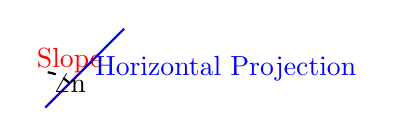
\begin{tikzpicture}
  % Set up 3D coordinates
  % Define the slope as a line from (0,0,0) to (1,1,1)
  % The angle n is the angle between the slope and the horizontal plane
  % First, draw the horizontal plane (xy-plane) and the slope
  % Draw the slope line
  \draw[thick, red] (0,0,0) -- (1,1,1) node[midway, above] {Slope};
  % Draw the horizontal projection of the slope
  \draw[thick, blue] (0,0,0) -- (1,1,0) node[midway, right] {Horizontal Projection};
  % Draw the angle between the slope and its horizontal projection
  % The angle is n, so label it
  \draw[thick, dashed] (0.5,0.5,0.5) arc[start angle=45, end angle=90, radius=0.5];
  \node at (0.5,0.5,0.5) {\angle n};
\end{tikzpicture}

\end{document}